\documentclass[conference]{IEEEtran}
\usepackage[T1]{fontenc}
\usepackage{cite}
\usepackage{amsmath,amssymb}
\usepackage{graphicx}
\usepackage[hidelinks]{hyperref}
\usepackage{url}

\title{TrueTone: Multimodal Sarcasm Detection Using Text and Speech Prosody}
\author{
\IEEEauthorblockN{Manas Sharma, Raghav Vats, Vaibhav Singh, and Sumit Bhati}
\IEEEauthorblockA{CSE Artificial Intelligence, Bennett University, Greater Noida, India\\
Enrolments, respectively: S24CSEU2420, S24CSEU1665, S24CSEU1668, S24CSEU2870}
}
\begin{document}
\maketitle

\begin{abstract}
A transcript can preserve a speaker's words while losing the tone that changes their meaning. TrueTone examines whether speech representations and prosodic features improve sarcasm detection beyond text alone, and whether an explicit text--tone mismatch representation adds further value. We evaluate frozen text, sentiment, speech, and emotion encoders with logistic regression and a gated fusion network on 690 balanced MUStARD utterances. Repeated stratified five-fold cross-validation gives the gated multimodal model a mean sarcastic-class F1 of 0.765, compared with 0.662 for its text baseline. Performance drops when complete television shows are held out. Speech-based logistic regression achieves the highest pooled cross-show F1 of 0.658, while gated fusion with mismatch achieves 0.648. Removing mismatch slightly reduces the network's random-split F1 but improves its cross-show F1. These findings support combining text and speech for random-split detection, while showing that explicit mismatch features do not provide a consistent generalisation benefit.
\end{abstract}
\begin{IEEEkeywords}
sarcasm detection, multimodal learning, speech prosody, gated fusion, MUStARD
\end{IEEEkeywords}

\section{Introduction}
The phrase ``Wonderful, another meeting'' can express approval or frustration. Its transcript alone does not establish which interpretation the speaker intends. Pitch, energy, timing, and surrounding dialogue may change how the same words are understood. Sarcasm detection therefore provides a useful setting for examining what speech contributes to language classification.

TrueTone asks a specific question: does adding speech help most when a speaker's tone appears to contradict the words? We separate this question into two comparisons. First, we compare text-based models with models that also receive speech features. Second, we compare fusion with and without explicit mismatch features. This distinction matters because a stronger multimodal model does not, by itself, demonstrate that mismatch explains the improvement.

Our implementation uses pretrained encoders without fine-tuning their weights. It combines RoBERTa text embeddings, WavLM speech embeddings, hand-crafted prosody, and sentiment/emotion probabilities. We compare logistic regression (LR) with a small gated network (NET), then remove feature blocks to examine their contribution. The experiment uses the original MUStARD dataset \cite{castro2019}. We report both random utterance splits and held-out-show tests, since a model can exploit recurring speakers or recording conditions when these are shared between training and test data.

The main contribution is an implemented comparison of unimodal references, early fusion, and feature-block gating, together with an explicit mismatch ablation. The results show a clear random-split advantage over text alone. They also show why this advantage should not be treated as evidence that mismatch is a reliable cue across unseen shows.

\section{Related Work}
Castro et al. introduced MUStARD, a collection of television utterances with transcripts, audiovisual clips, context, and sarcasm annotations \cite{castro2019}. Their work motivates the use of cues beyond text. Ray et al. extended this line of work through MUStARD++, adding emotion annotations for studying emotion in sarcastic speech \cite{ray2022}. Bhosale et al. benchmarked MUStARD++ and introduced a balanced extension with additional data \cite{bhosale2023}. These are related datasets and research directions. The experiments in this paper use the 690-utterance original MUStARD release, rather than either extension.

RoBERTa provides pretrained language representations \cite{liu2019}. We use its large variant to encode utterances and a separate CardiffNLP sentiment checkpoint for negative, neutral, and positive probabilities \cite{cardiff}. WavLM provides pretrained speech representations \cite{chen2022}. Speech emotion probabilities come from a wav2vec 2.0 checkpoint for the SUPERB emotion-recognition task \cite{yang2021,superber}. These encoders supply complementary feature blocks, but their outputs do not directly establish sarcastic intent.

Hand-crafted prosody provides a smaller representation of how an utterance sounds. Our pitch features use probabilistic YIN (pYIN) \cite{mauch2014}. We combine pitch with energy, timing, spectral features, and mel-frequency cepstral coefficients. The purpose is to test their contribution alongside learned speech embeddings, rather than assume that any particular acoustic pattern uniquely identifies sarcasm.

\section{Data and Preprocessing}
MUStARD contains 690 utterances, split evenly between sarcastic and non-sarcastic labels. The clips come from \emph{Friends} (356), \emph{The Big Bang Theory} (280), \emph{The Golden Girls} (40), and \emph{Sarcasmaholics Anonymous} (14). Class balance differs substantially across shows: 39 of the 40 \emph{Golden Girls} clips and all 14 \emph{Sarcasmaholics Anonymous} clips are sarcastic.

We download the annotations from the dataset repository and match each utterance identifier to its video clip. Audio is extracted as 16 kHz mono PCM. The mean clip duration is approximately 5.2 seconds. Audio feature extraction uses at most the first 30 seconds of each clip. The encoders pad very short signals as needed. Video frames are not used. Dialogue context enters only the text-with-context ablation; the main models use the target utterance.

Feature arrays are cached so that the repeated classifier fits reuse the same frozen representations. Training-fold preprocessing is applied separately for each outer evaluation split.

\section{Methodology}
\subsection{Text and Speech Representations}
The utterance text is encoded with \texttt{roberta-large}. We average the final hidden states over non-padding tokens, obtaining 1,024 features. A separate CardiffNLP Twitter-RoBERTa sentiment model returns three probabilities \cite{cardiff}. For the context ablation, RoBERTa receives an utterance--context pair.

The audio encoder is \texttt{microsoft/wavlm-large}. We average the hidden states from the middle third of its transformer layers, then concatenate temporal means and standard deviations to form a 2,048-dimensional vector. The emotion model, \texttt{superb/wav2vec2-base-superb-er}, produces probabilities over neutral, happy, angry, and sad speech \cite{superber}. All four pretrained models remain frozen.

We also extract 58 prosodic and acoustic features. These include voiced-frame proportion, pitch statistics, pitch slope, energy statistics, pause counts and durations, onset rates, spectral measures, and 13 MFCC means and standard deviations. Speaking and articulation rates use transcript word counts divided by clip duration or detected active-speech duration. Consequently, the configurations named ``speech-only'' and ``prosody-only'' are not entirely independent of text. We retain these implementation names while making the dependence explicit. Jitter and shimmer measures are frame-level proxies, not clinical voice-quality measurements.

\subsection{Text--Tone Mismatch}
Let the sentiment probabilities be $p_{\mathrm{neg}}$, $p_{\mathrm{neu}}$, and $p_{\mathrm{pos}}$. Text valence is
\begin{equation}
v_t = p_{\mathrm{pos}} - p_{\mathrm{neg}}.
\end{equation}
With emotion probabilities $q_k$, speech valence is
\begin{equation}
v_s = \sum_k q_k a_k,
\end{equation}
where $a_{\mathrm{happy}}=1$, $a_{\mathrm{angry}}=a_{\mathrm{sad}}=-1$, and $a_{\mathrm{neutral}}=0$. This mapping is a modelling assumption: it reduces emotion to a coarse valence estimate.

The six mismatch features are
\begin{equation}
\mathbf{m} = [v_t,v_s,v_t-v_s,|v_t-v_s|,v_tv_s,f],
\end{equation}
where $f=1$ only when the valences have opposite signs and both magnitudes exceed 0.1. Otherwise $f=0$. These features describe disagreement between two pretrained predictors. They should not be interpreted as ground-truth annotations of contradiction.

\subsection{Classifiers and Feature Blocks}
Text models receive text embeddings and sentiment probabilities. Speech models receive WavLM, prosody, and emotion features. Multimodal models receive both groups, with mismatch added where specified. Early fusion concatenates the selected blocks.

For LR, we standardise each block using the outer training fold, clip transformed values to $[-5,5]$, and scale each block by $1/\sqrt{d}$, where $d$ is its dimensionality. Balanced class weights address changes in class proportions across folds. An inner three-fold stratified search selects the inverse regularisation strength from $\{0.1,0.5,2,10,50,300,1000\}$ using log loss. Outer test examples never enter the scaler fit. However, preprocessing precedes the inner search, so its inner validation folds are not fully isolated from preprocessing statistics.

The gated network projects each block into 128 dimensions with dropout, a linear layer, layer normalisation, and GELU activation. A softmax gate assigns an example-specific weight to each projected block. Their weighted sum passes to a small classification head. Thus the gate operates over feature blocks, not simply one text branch and one audio branch.

We train with AdamW, a learning rate of $10^{-3}$, weight decay of $10^{-2}$, dropout of 0.4, label smoothing of 0.1, and a one-cycle schedule. Each fit uses 60 epochs and batches of 64. Predictions average three seeded networks. These settings are fixed in the notebook rather than selected on the outer test folds. There are 14 named model variants. LR early fusion and the LR no-mismatch ablation are identical configurations, so their matching scores are expected.

\begin{table*}[t]
\caption{Main results on MUStARD. CV entries are means over 15 folds; the CV F1 column includes fold standard deviations. Cross-show metrics pool the 636 held-out utterances. F1 uses sarcasm as the positive class.}
\label{tab:main}
\centering
\begin{tabular}{lccccc}
\hline
Model & CV accuracy & CV F1 (mean $\pm$ SD) & Cross-show accuracy & Cross-show F1 & Cross-show macro-F1 \\
\hline
LR text & 0.660 & 0.669 $\pm$ 0.040 & 0.538 & 0.580 & 0.533 \\
LR speech & 0.719 & 0.727 $\pm$ 0.042 & 0.612 & \textbf{0.658} & 0.604 \\
LR early fusion & 0.736 & 0.743 $\pm$ 0.049 & 0.601 & 0.644 & 0.595 \\
LR fusion + mismatch & 0.735 & 0.742 $\pm$ 0.048 & 0.604 & 0.645 & 0.598 \\
NET text & 0.662 & 0.662 $\pm$ 0.044 & 0.550 & 0.598 & 0.544 \\
NET speech & 0.720 & 0.721 $\pm$ 0.037 & 0.582 & 0.637 & 0.572 \\
NET gated + mismatch & 0.761 & \textbf{0.765 $\pm$ 0.048} & 0.594 & 0.648 & 0.585 \\
NET gated, no mismatch & 0.756 & 0.760 $\pm$ 0.052 & 0.602 & 0.656 & 0.592 \\
\hline
\end{tabular}
\end{table*}


\section{Experimental Setup}
\subsection{Evaluation Protocols}
Protocol A is repeated stratified five-fold CV with three repeats and random seed 42. Each model has 15 fold-level results. Speakers and shows can occur in both training and test sets, so this protocol measures performance within the available mixture of shows.

Protocol B holds out each eligible show in turn. A show must contain at least ten examples of each class to serve as a test fold. This selects \emph{The Big Bang Theory} and \emph{Friends}, yielding 636 pooled held-out utterances. The other two shows remain in training. We report pooled metrics for this protocol rather than mixing pooled F1 with the unweighted mean of show-level F1.

Sarcasm is the positive class, and all predictions use a probability threshold of 0.5. We report accuracy, positive-class F1, and macro-F1. CV standard deviations describe variation over overlapping folds; they are not standard errors from independent experiments. We do not compare these numbers directly with published systems that use different data or split rules.

\begin{figure*}[t]
\centering
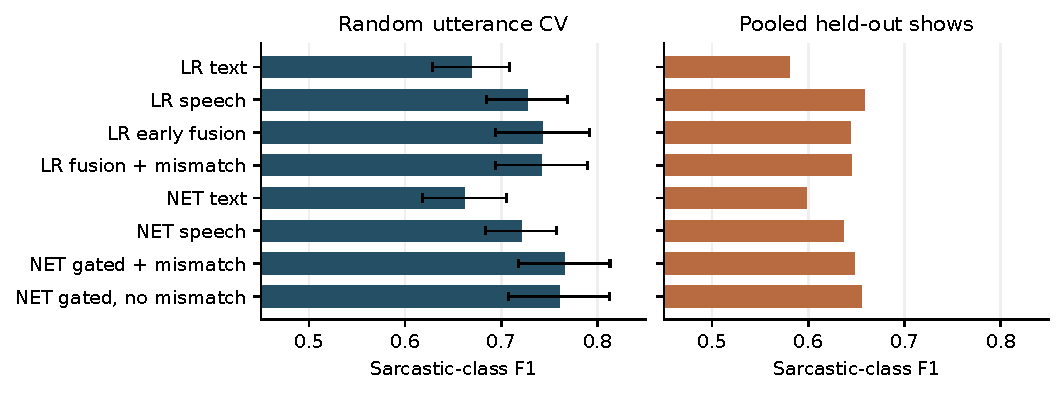
\includegraphics[width=\textwidth]{figures/model-comparison.pdf}
\caption{The model ranking changes across evaluation protocols. Left: mean CV F1 with fold-standard-deviation error bars. Right: pooled held-out-show F1, without error bars. The two panels use different aggregation rules and should be read as separate evaluations.}
\label{fig:comparison}
\end{figure*}

\subsection{Mismatch Analysis and Reproducibility}
For descriptive analysis, we divide examples into tertiles of $|v_t-v_s|$ and examine polarity-flip subsets. These analyses use the first CV repeat's out-of-fold predictions. Exploratory paired bootstrap intervals use 2,000 utterance resamples from the same repeat, or from the pooled cross-show predictions. They therefore describe a different quantity from the mean F1 over all 15 CV folds. Shared speakers and shows also weaken the bootstrap's independence assumption.

The complete corrected notebook ran on a local macOS arm64 CPU with four classifier workers in 10.8 minutes, including setup and downloads. The environment used Python 3.12.14, PyTorch 2.15.0, Transformers 5.23.0, librosa 1.0.1, and scikit-learn 1.9.1. All 15 code cells completed. The repository records the executed notebook, exact tables, and dependency versions \cite{truetone}. Pretrained checkpoint revisions are not pinned, so a future download may differ.



\section{Results and Discussion}
\subsection{Main Model Comparison}
Table~\ref{tab:main} reports results from the completed local run. Gated fusion with mismatch achieves the highest mean CV F1, 0.765, with a fold standard deviation of 0.048. Its text-only counterpart achieves 0.662, while speech-only NET reaches 0.721. LR also improves over its text baseline when speech is included: mean F1 rises from 0.669 for text to 0.743 for early fusion. These comparisons support the value of speech features in random utterance splits.

The cross-show ranking is different (Fig.~\ref{fig:comparison}). Speech LR leads with pooled F1 0.658 and accuracy 0.612. Gated fusion with mismatch obtains F1 0.648 and accuracy 0.594. The best random-split model is therefore not the strongest model under this cross-show test. The decline is consistent with sensitivity to show-specific speakers or acoustics, although the experiment does not isolate which factor causes it.

\subsection{Does Explicit Mismatch Help?}
Removing mismatch changes gated NET mean CV F1 from 0.765 to 0.760, a difference of approximately 0.005. On pooled cross-show evaluation, removal improves F1 from 0.648 to 0.656. The LR comparison is similarly modest: mean CV F1 is 0.742 with mismatch and 0.743 without it, while pooled cross-show F1 is 0.645 and 0.644, respectively. These results do not establish a consistent mismatch benefit.

The exploratory first-repeat bootstrap gives LR fusion minus text a CV F1 difference of 0.067, with interval $[0.032,0.101]$. For LR fusion minus speech, the difference is 0.007 with interval $[-0.019,0.032]$. On pooled cross-show predictions, LR fusion minus speech is $-0.013$ with interval $[-0.039,0.015]$. These intervals help describe the observed comparisons, but their sampling assumptions do not justify broad claims about unseen speakers or domains.

\begin{table}[t]
\caption{LR ablations. CV F1 is the mean over 15 folds. Cross-show F1 is pooled.}
\label{tab:ablations}
\centering
\begin{tabular}{lcc}
\hline
Feature configuration & CV F1 & Cross-show F1 \\
\hline
All blocks & 0.742 & 0.645 \\
Without mismatch & 0.743 & 0.644 \\
Without prosody & 0.747 & 0.624 \\
Without WavLM & 0.731 & 0.626 \\
Prosody only & 0.699 & 0.636 \\
Sentiment, emotion, mismatch & 0.624 & 0.607 \\
Text with context & 0.670 & 0.539 \\
\hline
\end{tabular}
\end{table}

\subsection{Feature Ablations and Contradiction Subsets}
Table~\ref{tab:ablations} shows that the feature contribution depends on the protocol. Removing prosody slightly raises LR CV F1 to 0.747 but reduces pooled cross-show F1 to 0.624. Removing WavLM gives 0.731 and 0.626, respectively. The small prosody-only LR model reaches pooled cross-show F1 0.636. Useful acoustic information is therefore present outside the learned speech embedding, but the experiments do not support a single feature ranking across both settings.

Average absolute text--tone disagreement is 0.542 for sarcastic clips and 0.621 for non-sarcastic clips. The uncorrected Mann--Whitney comparison gives $p=0.0504$. Polarity flips occur in 27.8\% of sarcastic examples and 30.4\% of non-sarcastic examples. Neither descriptive statistic supports the simple rule that sarcastic speech must have greater sentiment--emotion disagreement.

Subset comparisons can still show a fusion advantage over text, but this is distinct from proving that the explicit mismatch block causes that advantage. The subset analysis is exploratory, uses one CV repeat, and inherits any error in the pretrained sentiment and emotion predictors.

\section{Limitations and Future Work}
The dataset is small and consists of scripted television speech. Laugh tracks, channel characteristics, and recurring speakers can provide shortcuts that do not transfer to ordinary conversation. Holding out two shows is a useful stress test, but it is not a general evaluation across domains. The nearly single-class shows remaining in training further complicate interpretation.

The sentiment model is trained for a different text domain, and the emotion model represents acted emotional speech. Their valence estimates may be poorly calibrated for sarcasm. The mapping from happy/angry/sad/neutral to scalar valence also discards information. Transcript-derived rate features prevent a strict audio-only interpretation of the speech references.

Statistical conclusions are limited by correlated utterances, overlapping CV folds, and exploratory feature comparisons. Inner-CV preprocessing should be moved into the tuning pipeline for stricter isolation. Future work should also use speaker-aware splits, assess calibration, and pin immutable model revisions. A separate evaluation on MUStARD++ would allow a closer study of its emotion annotations and a broader comparison of mismatch representations.

\section{Conclusion}
TrueTone combines frozen text and speech encoders with prosody and explicit text--tone mismatch features. On the original MUStARD dataset, gated fusion achieves mean random-split F1 0.765 and improves over its text baseline. The held-out-show evaluation gives a different result: speech LR leads with pooled F1 0.658, and explicit mismatch does not consistently improve generalisation. The main practical finding is that the evaluation split changes the conclusion about which model is strongest. Future comparisons should preserve that distinction and test mismatch against matched no-mismatch baselines.

\section*{Acknowledgment}
The authors thank Dr. Saurabh Kumar Srivastava for project guidance.

\bibliographystyle{IEEEtran}
\bibliography{references}
\end{document}
